% Options for packages loaded elsewhere
\PassOptionsToPackage{unicode}{hyperref}
\PassOptionsToPackage{hyphens}{url}
\PassOptionsToPackage{dvipsnames,svgnames,x11names}{xcolor}
%
\documentclass[
  letterpaper,
  DIV=11,
  numbers=noendperiod]{scrartcl}

\usepackage{amsmath,amssymb}
\usepackage{iftex}
\ifPDFTeX
  \usepackage[T1]{fontenc}
  \usepackage[utf8]{inputenc}
  \usepackage{textcomp} % provide euro and other symbols
\else % if luatex or xetex
  \usepackage{unicode-math}
  \defaultfontfeatures{Scale=MatchLowercase}
  \defaultfontfeatures[\rmfamily]{Ligatures=TeX,Scale=1}
\fi
\usepackage{lmodern}
\ifPDFTeX\else  
    % xetex/luatex font selection
  \setmainfont[]{Atkinson Hyperlegible}
  \setsansfont[]{Atkinson Hyperlegible}
  \setmonofont[]{Fira Code}
\fi
% Use upquote if available, for straight quotes in verbatim environments
\IfFileExists{upquote.sty}{\usepackage{upquote}}{}
\IfFileExists{microtype.sty}{% use microtype if available
  \usepackage[]{microtype}
  \UseMicrotypeSet[protrusion]{basicmath} % disable protrusion for tt fonts
}{}
\makeatletter
\@ifundefined{KOMAClassName}{% if non-KOMA class
  \IfFileExists{parskip.sty}{%
    \usepackage{parskip}
  }{% else
    \setlength{\parindent}{0pt}
    \setlength{\parskip}{6pt plus 2pt minus 1pt}}
}{% if KOMA class
  \KOMAoptions{parskip=half}}
\makeatother
\usepackage{xcolor}
\setlength{\emergencystretch}{3em} % prevent overfull lines
\setcounter{secnumdepth}{-\maxdimen} % remove section numbering
% Make \paragraph and \subparagraph free-standing
\ifx\paragraph\undefined\else
  \let\oldparagraph\paragraph
  \renewcommand{\paragraph}[1]{\oldparagraph{#1}\mbox{}}
\fi
\ifx\subparagraph\undefined\else
  \let\oldsubparagraph\subparagraph
  \renewcommand{\subparagraph}[1]{\oldsubparagraph{#1}\mbox{}}
\fi


\providecommand{\tightlist}{%
  \setlength{\itemsep}{0pt}\setlength{\parskip}{0pt}}\usepackage{longtable,booktabs,array}
\usepackage{calc} % for calculating minipage widths
% Correct order of tables after \paragraph or \subparagraph
\usepackage{etoolbox}
\makeatletter
\patchcmd\longtable{\par}{\if@noskipsec\mbox{}\fi\par}{}{}
\makeatother
% Allow footnotes in longtable head/foot
\IfFileExists{footnotehyper.sty}{\usepackage{footnotehyper}}{\usepackage{footnote}}
\makesavenoteenv{longtable}
\usepackage{graphicx}
\makeatletter
\def\maxwidth{\ifdim\Gin@nat@width>\linewidth\linewidth\else\Gin@nat@width\fi}
\def\maxheight{\ifdim\Gin@nat@height>\textheight\textheight\else\Gin@nat@height\fi}
\makeatother
% Scale images if necessary, so that they will not overflow the page
% margins by default, and it is still possible to overwrite the defaults
% using explicit options in \includegraphics[width, height, ...]{}
\setkeys{Gin}{width=\maxwidth,height=\maxheight,keepaspectratio}
% Set default figure placement to htbp
\makeatletter
\def\fps@figure{htbp}
\makeatother
% definitions for citeproc citations
\NewDocumentCommand\citeproctext{}{}
\NewDocumentCommand\citeproc{mm}{%
  \begingroup\def\citeproctext{#2}\cite{#1}\endgroup}
\makeatletter
 % allow citations to break across lines
 \let\@cite@ofmt\@firstofone
 % avoid brackets around text for \cite:
 \def\@biblabel#1{}
 \def\@cite#1#2{{#1\if@tempswa , #2\fi}}
\makeatother
\newlength{\cslhangindent}
\setlength{\cslhangindent}{1.5em}
\newlength{\csllabelwidth}
\setlength{\csllabelwidth}{3em}
\newenvironment{CSLReferences}[2] % #1 hanging-indent, #2 entry-spacing
 {\begin{list}{}{%
  \setlength{\itemindent}{0pt}
  \setlength{\leftmargin}{0pt}
  \setlength{\parsep}{0pt}
  % turn on hanging indent if param 1 is 1
  \ifodd #1
   \setlength{\leftmargin}{\cslhangindent}
   \setlength{\itemindent}{-1\cslhangindent}
  \fi
  % set entry spacing
  \setlength{\itemsep}{#2\baselineskip}}}
 {\end{list}}
\usepackage{calc}
\newcommand{\CSLBlock}[1]{\hfill\break\parbox[t]{\linewidth}{\strut\ignorespaces#1\strut}}
\newcommand{\CSLLeftMargin}[1]{\parbox[t]{\csllabelwidth}{\strut#1\strut}}
\newcommand{\CSLRightInline}[1]{\parbox[t]{\linewidth - \csllabelwidth}{\strut#1\strut}}
\newcommand{\CSLIndent}[1]{\hspace{\cslhangindent}#1}

\usepackage{fancyhdr}
\pagestyle{fancy}
\fancyfoot[C]{\thepage}
\renewcommand{\headrulewidth}{0.4pt}
\renewcommand{\footrulewidth}{0.4pt}
\KOMAoption{captions}{tableheading}
\makeatletter
\@ifpackageloaded{caption}{}{\usepackage{caption}}
\AtBeginDocument{%
\ifdefined\contentsname
  \renewcommand*\contentsname{Table of contents}
\else
  \newcommand\contentsname{Table of contents}
\fi
\ifdefined\listfigurename
  \renewcommand*\listfigurename{List of Figures}
\else
  \newcommand\listfigurename{List of Figures}
\fi
\ifdefined\listtablename
  \renewcommand*\listtablename{List of Tables}
\else
  \newcommand\listtablename{List of Tables}
\fi
\ifdefined\figurename
  \renewcommand*\figurename{Figure}
\else
  \newcommand\figurename{Figure}
\fi
\ifdefined\tablename
  \renewcommand*\tablename{Table}
\else
  \newcommand\tablename{Table}
\fi
}
\@ifpackageloaded{float}{}{\usepackage{float}}
\floatstyle{ruled}
\@ifundefined{c@chapter}{\newfloat{codelisting}{h}{lop}}{\newfloat{codelisting}{h}{lop}[chapter]}
\floatname{codelisting}{Listing}
\newcommand*\listoflistings{\listof{codelisting}{List of Listings}}
\makeatother
\makeatletter
\makeatother
\makeatletter
\@ifpackageloaded{caption}{}{\usepackage{caption}}
\@ifpackageloaded{subcaption}{}{\usepackage{subcaption}}
\makeatother
\ifLuaTeX
  \usepackage{selnolig}  % disable illegal ligatures
\fi
\usepackage{bookmark}

\IfFileExists{xurl.sty}{\usepackage{xurl}}{} % add URL line breaks if available
\urlstyle{same} % disable monospaced font for URLs
\hypersetup{
  pdftitle={Lecture 13:   Philosophy of Science},
  pdfauthor={Dr.~Gordon Wright},
  colorlinks=true,
  linkcolor={blue},
  filecolor={Maroon},
  citecolor={Blue},
  urlcolor={Blue},
  pdfcreator={LaTeX via pandoc}}

\title{Lecture 13: Philosophy of Science}
\usepackage{etoolbox}
\makeatletter
\providecommand{\subtitle}[1]{% add subtitle to \maketitle
  \apptocmd{\@title}{\par {\large #1 \par}}{}{}
}
\makeatother
\subtitle{An initial overview}
\author{Dr.~Gordon Wright}
\date{January 8, 2024}

\begin{document}
\maketitle

\raggedright

\section{Is Psychology a Science?}\label{is-psychology-a-science}

\subsection{The Ongoing Debate}\label{the-ongoing-debate}

\begin{itemize}
\tightlist
\item
  \textbf{Positivism in Psychology}: Traditional view supporting
  quantitative methods, treating human behavior as stable, measurable
  facts.
\item
  \textbf{Qualitative Shift}: A focus on dynamic, ever-changing aspects
  of human behavior, challenging the idea of fixed patterns, and
  possibly facts!
\item
  Source: (\textbf{parker2011?})
\end{itemize}

\subsection{The Role of Qualitative
Research}\label{the-role-of-qualitative-research}

\begin{itemize}
\tightlist
\item
  \textbf{Qualitative vs.~Quantitative}: The debate isn't about the
  validity of quantification but the quality of its application in
  psychology.
\item
  Where is Psychology's non-stick frying pan? (Banyard, 2015)
\item
  \textbf{Advancing Scientific Debate}: Qualitative research is at the
  forefront of discussions about the nature of scientific inquiry in
  psychology.
\item
  Source: (Parker, 2004)
\end{itemize}

\section{The Structure of Scientific
Revolutions}\label{the-structure-of-scientific-revolutions}

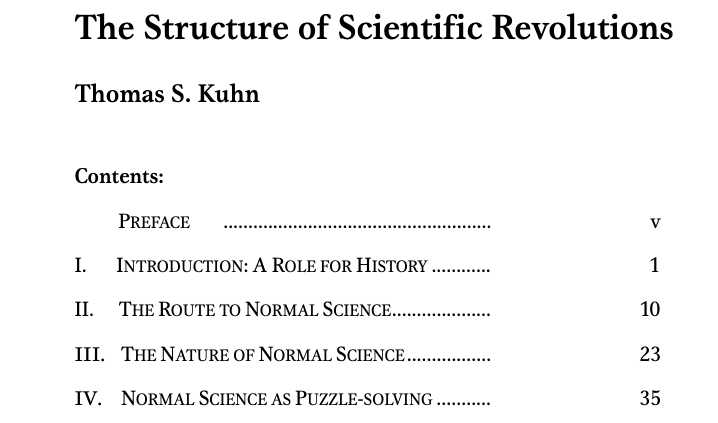
\includegraphics[width=5.20833in,height=\textheight]{images/Kuhn.png}

\href{https://folk.ntnu.no/krill/bioko-references/Kuhn\%201962.pdf}{Kuhn
- Structure}

\subsection{Paradigm Shifts}\label{paradigm-shifts}

\begin{itemize}
\item
  \textbf{Thomas Kuhn's Theory}: Science progresses through paradigm
  shifts rather than linear accumulation of knowledge.
\item
  \textbf{Application in Psychology}: Shifts from behaviorism to
  cognitive psychology, and then to more integrated approaches.

  \begin{figure}[H]

  {\centering 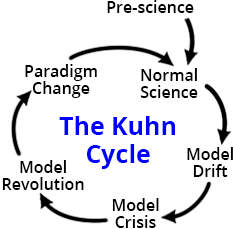
\includegraphics{lecture_files/mediabag/KuhnCycle_BasicCycle.png}

  }

  \caption{The Kuhn Cycle - Thomas Kuhn\textquotesingle s Brilliant
  Model of How Scientific Fields Progress}

  \end{figure}%
\end{itemize}

\subsection{Implications for Psychological
Research}\label{implications-for-psychological-research}

\begin{itemize}
\tightlist
\item
  \textbf{Changing Research Methods}: Embracing diverse methodologies
  reflecting evolving paradigms in psychology.
\item
  \textbf{Interdisciplinary Influence}: Incorporating insights from
  philosophy, sociology, and neuroscience into psychological research.
\end{itemize}

\subsection{Psychology as a `Soft
Science'}\label{psychology-as-a-soft-science}

\begin{itemize}
\tightlist
\item
  Psychology compared to pre-scientific stages of sciences
\item
  The debate over applying `the scientific method' in psychology
\item
  The importance of being phenomenon-centered and problem-centered
\item
  Misalignment of methods with research questions
\end{itemize}

Uher (2021)

\section{Conclusion?}\label{conclusion}

\subsection{Psychology and Science}\label{psychology-and-science}

\begin{itemize}
\tightlist
\item
  \textbf{Dynamic and Evolving}: Psychology, like other sciences,
  undergoes paradigm shifts and methodological evolution.
\item
  \textbf{Beyond Traditional Boundaries}: The discipline is increasingly
  recognizing the value of qualitative, subjective, and diverse
  approaches to understanding the human mind and behavior.
\end{itemize}

\begin{center}\rule{0.5\linewidth}{0.5pt}\end{center}

\section{Karl Popper and
Falsification}\label{karl-popper-and-falsification}

\subsection{The Principle of
Falsification}\label{the-principle-of-falsification}

\begin{itemize}
\tightlist
\item
  \textbf{Karl Popper's Contribution}: Emphasized the importance of
  falsifiability in scientific theories.
\item
  \textbf{Falsification vs.~Verification}: Popper argued that scientific
  theories can never be completely verified, but they can be falsified.
\item
  \textbf{Impact on Psychology}: Encourages rigorous testing of
  hypotheses and openness to disconfirming evidence in psychological
  research.
\end{itemize}

\subsection{Critiques and Legacy}\label{critiques-and-legacy}

\begin{itemize}
\tightlist
\item
  \textbf{Practical Challenges}: Difficulties in applying falsification
  principle in complex fields like psychology.
\item
  \textbf{Enduring Influence}: Popper's ideas continue to influence
  scientific methodology and philosophical discussions in psychology.
\end{itemize}

\section{Epistemology}\label{epistemology}

\subsection{Epistemology}\label{epistemology-1}

\begin{itemize}
\tightlist
\item
  \textbf{Definition}: The study of knowledge -- its nature, origin, and
  limits.
\item
  \textbf{Relevance to Psychology}: Helps in understanding how we
  acquire knowledge about human behavior and mental processes.
\item
  How do we know what we know, or get to know something new?
\end{itemize}

\section{\texorpdfstring{Understanding the
\textbf{Ideographic/Nomothetic}
Divide}{Understanding the Ideographic/Nomothetic Divide}}\label{understanding-the-ideographicnomothetic-divide}

\href{https://www.bps.org.uk/psychologist/looking-back-war-words}{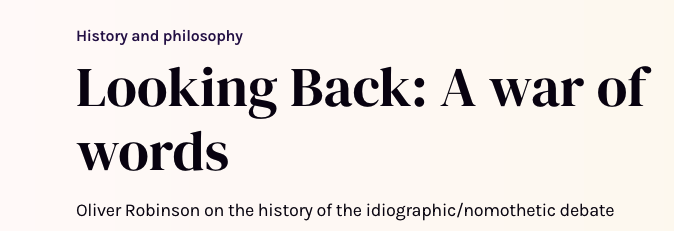
\includegraphics{images/Qual@2x.png}}

\subsection{Ideographic Approach}\label{ideographic-approach}

\begin{itemize}
\tightlist
\item
  \textbf{Focus}: Emphasizes the unique aspects of individual cases or
  phenomena.
\item
  \textbf{Methodology}: Often uses qualitative methods, such as case
  studies, to explore complex, subjective experiences.
\item
  \textbf{Goal}: To understand the depth and complexity of individual
  experiences.
\end{itemize}

\subsection{Nomothetic Approach}\label{nomothetic-approach}

\begin{itemize}
\tightlist
\item
  \textbf{Focus}: Seeks to identify general laws and patterns that apply
  across multiple cases.
\item
  \textbf{Methodology}: Employs quantitative methods, like experiments
  and surveys, to gather data on larger populations.
\item
  \textbf{Goal}: To formulate generalizations and broad theories
  applicable to many.
\end{itemize}

\section{Implications in Psychological
Research}\label{implications-in-psychological-research}

\subsection{Balancing Perspectives}\label{balancing-perspectives}

\begin{itemize}
\tightlist
\item
  \textbf{Integrating Approaches}: Both ideographic and nomothetic
  methods offer valuable insights; combining them can lead to a more
  holistic understanding of psychological phenomena.
\item
  \textbf{Challenges in Quantitative Research}: The need to acknowledge
  and address the reflexive capacity of human beings and the meaningful
  nature of data from aggregated descriptions of behavior.
\item
  \textbf{Innovative Research Possibilities}: Opportunities for
  innovative research that addresses these challenges, respecting the
  particularities of individual cases within broader patterns.
\item
  (Robinson, 2012)
\end{itemize}

\section{Why should we care about this
question?}\label{why-should-we-care-about-this-question}

\subsection{The Esteem of Science}\label{the-esteem-of-science}

\begin{itemize}
\tightlist
\item
  Science's high regard in society and academia
\item
  The assumption that the scientific method leads to reliable results
\item
  The challenge in defining `scientific method' and its transferability
\end{itemize}

\href{source}{\emph{Chalmers, 2014}} What is this thing called Science?

\begin{center}\rule{0.5\linewidth}{0.5pt}\end{center}

\subsection{Conclusion: Rethinking Scientific Method in
Psychology}\label{conclusion-rethinking-scientific-method-in-psychology}

\begin{itemize}
\tightlist
\item
  Recognizing the influence of subjective experiences on observation
\item
  Understanding the interplay between facts, theory, and conceptual
  frameworks
\item
  The challenge of applying a rigid scientific method to human behavior
  and experiences
\end{itemize}

\begin{center}\rule{0.5\linewidth}{0.5pt}\end{center}

\subsection{Abstract}\label{abstract}

\begin{itemize}
\tightlist
\item
  Psychology's struggle with foundational concepts: mind and behavior
\item
  Lack of unified theoretical framework
\item
  Classification as a `soft science'
\item
  Need for diverse methodologies and systematic integration
\item
  Galtonian nomothetic methodology's limitations
\end{itemize}

{[}\emph{Uher, 2020}{]}

\begin{center}\rule{0.5\linewidth}{0.5pt}\end{center}

\subsection{Lack of Proper Terms and
Definitions}\label{lack-of-proper-terms-and-definitions}

\begin{itemize}
\tightlist
\item
  Discordant and ambiguous definitions in psychology
\item
  Overlap between psychology, neuroscience, and philosophy
\item
  Proliferation of terms and constructs
\item
  Deeply fragmented theoretical landscape
\end{itemize}

{[}\emph{Uher, 2020}{]}

\begin{center}\rule{0.5\linewidth}{0.5pt}\end{center}

\subsection{Lack of Conceptual
Integration}\label{lack-of-conceptual-integration}

\begin{itemize}
\tightlist
\item
  Diversity of epistemologies, paradigms, and methodologies
\item
  Absence of a unified theory in psychology
\item
  Challenges with evolutionary psychology as an integrative framework
\item
  Speculative nature of evolutionary explorations in psychology
\end{itemize}

{[}\emph{Uher, 2020}{]}

\begin{center}\rule{0.5\linewidth}{0.5pt}\end{center}

\subsection{Psychology as a `Soft
Science'}\label{psychology-as-a-soft-science-1}

\begin{itemize}
\tightlist
\item
  Psychology compared to pre-scientific stages of sciences
\item
  The debate over applying `the scientific method' in psychology
\item
  The importance of being phenomenon-centered and problem-centered
\item
  Misalignment of methods with research questions
\end{itemize}

{[}\emph{Uher, 2020}{]}

\begin{center}\rule{0.5\linewidth}{0.5pt}\end{center}

\subsection{Experience in Psychology}\label{experience-in-psychology}

\begin{itemize}
\tightlist
\item
  The dual aspects of experience: objective content and subjective
  apprehension
\item
  Contrast between natural sciences and psychological approaches
\item
  Psychology's focus on immediate subjective experience
\item
  The role of agency, volition, value orientation, and teleology
\end{itemize}

{[}\emph{Uher, 2020}{]}

\begin{center}\rule{0.5\linewidth}{0.5pt}\end{center}

\subsection{Constructs in Science and Everyday
Psychology}\label{constructs-in-science-and-everyday-psychology}

\begin{itemize}
\tightlist
\item
  Challenges posed by the transient nature of experience
\item
  The interplay of constructs with everyday knowledge and language
\item
  The entification of constructs and overlooking their constructed
  nature
\item
  Differentiation between psychical and psychological phenomena
\end{itemize}

{[}\emph{Uher, 2020}{]}

\begin{center}\rule{0.5\linewidth}{0.5pt}\end{center}

\subsection{Psychology's Exceptional
Position}\label{psychologys-exceptional-position}

\begin{itemize}
\tightlist
\item
  Psychology at the intersection of sciences and philosophy
\item
  Exploration of diverse phenomena across human life
\item
  Requirement for a plurality of methodologies and epistemologies
\item
  Psychology as a non-unitary science due to its wide-ranging study
  phenomena
\end{itemize}

{[}\emph{Uher, 2020}{]}

\begin{center}\rule{0.5\linewidth}{0.5pt}\end{center}

\subsection{Idiographic and Nomothetic
Strategies}\label{idiographic-and-nomothetic-strategies}

\begin{itemize}
\tightlist
\item
  The uniqueness of immediate experience
\item
  The use of idiographic strategies for exploring individual cases
\item
  Limitations of Galtonian nomothetic methodology
\item
  The impact of natural-science principles on psychological research
\end{itemize}

{[}\emph{Uher, 2020}{]}

\begin{center}\rule{0.5\linewidth}{0.5pt}\end{center}

\subsection{Moving Beyond Conceptual
Deadlock}\label{moving-beyond-conceptual-deadlock}

\begin{itemize}
\tightlist
\item
  Introduction of the Transdisciplinary Philosophy-of-Science Paradigm
  (TPS-Paradigm)
\item
  Aiming for critical reflection and development of new theories
\item
  Integration of concepts from various disciplines
\item
  Focus on the individual as the central unit of analysis
\end{itemize}

{[}\emph{Uher, 2020}{]}

\begin{center}\rule{0.5\linewidth}{0.5pt}\end{center}

\subsection{Philosophical Framework of the
TPS-Paradigm}\label{philosophical-framework-of-the-tps-paradigm}

\begin{itemize}
\tightlist
\item
  Three sets of presuppositions about research on individuals
\item
  Human limitations in perception and conceptualization
\item
  Concept of individuals as complex, open, and nested systems
\item
  Application of complementarity in methodology
\end{itemize}

{[}\emph{Uher, 2020}{]}

\begin{center}\rule{0.5\linewidth}{0.5pt}\end{center}

\subsection{Metatheoretical Framework}\label{metatheoretical-framework}

\begin{itemize}
\tightlist
\item
  Formalization of phenomena's accessibility to human perception
\item
  Differentiation of various kinds of phenomena related to individuals
\item
  Integration and development of concepts across fields
\item
  Exploration of psychical phenomena and their connections
\end{itemize}

{[}\emph{Uher, 2020}{]}

\begin{center}\rule{0.5\linewidth}{0.5pt}\end{center}

\subsection{Methodological Framework}\label{methodological-framework}

\begin{itemize}
\tightlist
\item
  Concepts for matching methodology with phenomena
\item
  Development of methods for comparing individuals
\item
  Analysis of data generation and measurement practices
\item
  Application of metrological principles in psychological research
\end{itemize}

{[}\emph{Uher, 2020}{]}

\begin{center}\rule{0.5\linewidth}{0.5pt}\end{center}

\subsection*{References}\label{references}
\addcontentsline{toc}{subsection}{References}

\phantomsection\label{refs}
\begin{CSLReferences}{1}{0}
\bibitem[\citeproctext]{ref-banyard2015}
Banyard, P. (2015). Where is psychology's non-stick frying pan? In
\emph{BPS}.
\url{https://www.bps.org.uk/psychologist/where-psychologys-non-stick-frying-pan}

\bibitem[\citeproctext]{ref-parker2004}
Parker, I. (2004). \emph{Qualitative psychology: Introducing radical
research}. McGraw-Hill Education (UK).

\bibitem[\citeproctext]{ref-robinson2012a}
Robinson, O. C. (2012). Looking back: A war of words. In \emph{BPS}.
\url{https://www.bps.org.uk/psychologist/looking-back-war-words}

\bibitem[\citeproctext]{ref-uher2021}
Uher, J. (2021). Psychology{'}s Status as a Science: Peculiarities and
Intrinsic Challenges. Moving Beyond its Current Deadlock Towards
Conceptual Integration. \emph{Integrative Psychological and Behavioral
Science}, \emph{55}(1), 212--224.
\url{https://doi.org/10.1007/s12124-020-09545-0}

\end{CSLReferences}



\end{document}
